% ---------------------------------------------------------------------
% CAOS_LDA_HSI series, paper P5: preprint (target venue redacted)
%
% Title  : Post-hoc Interpretability of LDA on Hyperspectral Imagery:
%          SHAP Attributions, Counterfactual Topic Flips, and LLM-judge
%          Alignment under Token-Mass-Dispersion Asymmetry (LDA only)
% Target : redacted while the preprint circulates
% Class  : IEEEtran journal option
% Scope  : F-13 SHAP, F-22 counterfactual and F-15 alignment on the
%          V1..V20 LDA sweep; two local figures (dispersion mechanism,
%          F-15 vs vocabulary). Companion to P3 (V-sweep) and P4
%          (backbone factorial); the canonical equation set shared with
%          P3/P4 lives at ../../equations/canonical.tex.
% ---------------------------------------------------------------------

\documentclass[journal,a4paper,10pt]{IEEEtran}

\usepackage[utf8]{inputenc}
\usepackage[T1]{fontenc}
\usepackage{amsmath,amssymb,amsfonts}
\usepackage{dsfont}% \mathds{1}: indicator function in the canonical equation set
\usepackage{graphicx}
\usepackage{booktabs}
\usepackage{array}
\usepackage{multirow}
\usepackage{cite}
\usepackage{xcolor}
\usepackage[hyphens]{url}% long reference URLs may break at hyphens
\usepackage[hidelinks]{hyperref}

\graphicspath{{../../figures/}}

% IEEEtran hard-codes an em-dash after the abstract and index-terms names; the CAOS
% content standard (ADR-0067) excludes em-dashes, so the separator is a full stop.
\makeatletter
\def\abstract{\normalfont
    \if@twocolumn
      \@IEEEabskeysecsize\bfseries\textit{\abstractname}.\ \relax
    \else
      \bgroup\par\addvspace{0.5\baselineskip}\centering\vspace{-1.78ex}\@IEEEabskeysecsize\textbf{\abstractname}\par\addvspace{0.5\baselineskip}\egroup\quotation\@IEEEabskeysecsize
    \fi\@IEEEgobbleleadPARNLSP}
\def\IEEEkeywords{\normalfont
    \if@twocolumn
      \@IEEEabskeysecsize\bfseries\textit{\IEEEkeywordsname}.\ \relax
    \else
      \bgroup\par\addvspace{0.5\baselineskip}\centering\@IEEEabskeysecsize\textbf{\IEEEkeywordsname}\par\addvspace{0.5\baselineskip}\egroup\quotation\@IEEEabskeysecsize
    \fi\@IEEEgobbleleadPARNLSP}
\makeatother

% Page-1 header block (conventions/manuscript-header-standard.md). The four document
% macros are set by the publishing tool when the version DOI is reserved.
\newcommand{\doctype}{Preprint}
\newcommand{\docversion}{v1.4}
\newcommand{\docdate}{19 September 2026}
\newcommand{\versiondoi}{10.5281/zenodo.22850133}
\newcommand{\conceptdoi}{10.5281/zenodo.21504113}
\newcommand{\docrepo}{github.com/fsantibanezleal/CAOS\_LDA\_HSI}
\newcommand{\headerblock}{%
\begin{center}
\fbox{\parbox{0.94\textwidth}{\small\raggedright
\textbf{\doctype} \quad$\cdot$\quad \docversion, \docdate \quad$\cdot$\quad Licence CC BY 4.0\\[2pt]
CAOS open-research programme \quad$\cdot$\quad CAOS\_LDA\_HSI, topic models on hyperspectral imagery (paper P5)\\[2pt]
Version DOI \href{https://doi.org/\versiondoi}{\texttt{\versiondoi}} \quad$\cdot$\quad
concept DOI (always latest) \href{https://doi.org/\conceptdoi}{\texttt{\conceptdoi}}\\[2pt]
Not peer reviewed. Source code, data and computational records: \href{https://\docrepo}{\texttt{\docrepo}}
}}
\end{center}}

\title{Post-hoc Interpretability of LDA on Hyperspectral Imagery:
SHAP Attributions, Counterfactual Topic Flips, and LLM-judge
Alignment under Token-Mass-Dispersion Asymmetry}

\author{%
  Felipe Santib\'a\~nez-Leal~\orcidlink{0000-0002-0150-3246},~\IEEEmembership{Independent Researcher}%
  \thanks{F.\ Santib\'a\~nez-Leal is with the CAOS open-research
    programme, Santiago, Chile
    (e-mail: \texttt{fsantibanezleal@ug.uchile.cl};
    ORCID: 0000-0002-0150-3246).}%
  \thanks{Companion papers: P3~\cite{santibanezleal2026sweep}
    (V-sweep) and P4~\cite{santibanezleal2026factorial} (backbone
    factorial). This study restricts the analysis to the
    \emph{latent Dirichlet allocation (LDA) backbone only}. Code and
    derived artefacts at
    \url{https://github.com/fsantibanezleal/CAOS_LDA_HSI}.}%
  \thanks{Partially funded by AMTC Basal (ANID/PIA AFB220002) and
    ANID FONDECYT Postdoctorado 3220094.}%
}

\markboth{\doctype\ \docversion, 2026 \textperiodcentered\ CAOS open-research programme}{Santib\'a\~nez-Leal:
Post-hoc Interpretability of LDA-on-HSI (LDA only)}

\IEEEaftertitletext{\vspace{-0.6\baselineskip}\headerblock\vspace{0.2\baselineskip}}

\IEEEtitleabstractindextext{%
\begin{abstract}
The interpretability claim of LDA-on-HSI rests on the assumption that
topic--word distributions are human-readable. \emph{This study is
restricted to the LDA backbone}; the cross-backbone comparison (HDP,
ProdLDA, ETM) is the subject of the companion paper
P4~\cite{santibanezleal2026factorial}. We test three
orthogonal post-hoc interpretability axes on the V1--V15, V17--V20
wordification sweep (nineteen LDA-fitted recipes) from the companion
paper P3~\cite{santibanezleal2026sweep}: F-13 SHAP attribution of pixel-to-topic decisions via a
closed-form posterior, F-22 counterfactual $L_1$ perturbation required
to flip a document's argmax topic, and F-15 LLM-as-judge alignment
between a document's top tokens and its argmax topic's top tokens.
We find three concrete results. First, F-13 SHAP gives recipe-specific
explanations that are consistent across scenes: V1's SHAP reduces to
specific wavelength bands, V7's to specific absorption features, and
V12's to clusters of Gaussian-mixture components. Second, F-22
counterfactual L1 (sentinel-patched 19-recipe ranking) separates the
recipes into an ``ultra-robust'' band (V20, V12, V3; sentinel-patched
means 26.3 / 24.5 / 23.5), a ``moderate'' band (V1 = 6.1, V7 = 5.2)
and a ``fragile'' band (V9 = 1.0, V10 = 1.2); within the ultra-robust
band a large fraction of documents never flip within 50 steps, so the
ordering is not strict (V12 is the most robust where flip-sampling is adequate).
Third, F-15, computed with a deterministic stand-in for the LLM judge,
is governed by how its top-10 overlap rule reads each recipe's
documents rather than by agreement between documents and topics. It is
1.0 by construction for V2 and V8 (at most 12 word types, so a topic's
top-10 covers the vocabulary) and for V9 (a one-token document can be
judged aligned or ambiguous but never misaligned), and stays near 1.0
for recipes with three or four tokens per document. Where a document
holds each of its tokens once, its top-10 is a tie, so we report the
exact expectation of the rule under uniformly random tie-breaking
rather than one sort order: V3 and V12 then score 0.17, against 0.03 to
0.18 across individual orders. V20 re-weights
V3's identical $(\mathrm{band},\mathrm{bin})$ alphabet and scores 0.65;
its topics are also less dispersed
(effective vocabulary $N_{\mathrm{eff}}=\exp\!\big(H(\phi_k)\big)$ of
309 against 431 for V3 and 400 for V12), but its per-band copies also
make each document's top-10 its highest-copy bands, so the comparison
cannot attribute the gap to topic dispersion. F-15 as defined therefore
measures the documents' token structure more than topic
interpretability, and an LLM oracle given the same token lists would
face the same construction effects. We recommend reporting F-13 SHAP
top-$K$ attributions as the primary interpretability artefact, F-22 as
the topic-stability artefact, and F-15 only with its construction
effects reported beside it.
\end{abstract}

\begin{IEEEkeywords}
hyperspectral imagery, latent Dirichlet allocation, post-hoc
interpretability, SHAP, counterfactual explanations, LLM-as-judge,
topic models, wordification, evaluation framework.
\end{IEEEkeywords}}

\usepackage[hidelinks]{hyperref}
\usepackage{orcidlink}

\begin{document}
\bstctlcite{IEEEexample:BSTcontrol}

\maketitle
\IEEEdisplaynontitleabstractindextext
\IEEEpeerreviewmaketitle

% ---------------------------------------------------------------------
% Canonical equation set, shared verbatim across P3/P4/P5. We \input the
% whole file; only the labels actually \eqref'd below are referenced.
% Authored once at ../../equations/canonical.tex (compiles clean).
% ---------------------------------------------------------------------
% ===================================================================
% CANONICAL EQUATION SET: CAOS_LDA_HSI manuscript series (P3/P4/P5)
% ===================================================================
% Single source of truth for all display equations. Authored once,
% \input into P3 (journal_v_sweep), P4 (journal_backbone_factorial),
% P5 (journal_interpretability), and transcribed (KaTeX) into the
% web-app methodology route and the wiki Mathematical-Background page.
%
% Usage:  % ===================================================================
% CANONICAL EQUATION SET: CAOS_LDA_HSI manuscript series (P3/P4/P5)
% ===================================================================
% Single source of truth for all display equations. Authored once,
% \input into P3 (journal_v_sweep), P4 (journal_backbone_factorial),
% P5 (journal_interpretability), and transcribed (KaTeX) into the
% web-app methodology route and the wiki Mathematical-Background page.
%
% Usage:  % ===================================================================
% CANONICAL EQUATION SET: CAOS_LDA_HSI manuscript series (P3/P4/P5)
% ===================================================================
% Single source of truth for all display equations. Authored once,
% \input into P3 (journal_v_sweep), P4 (journal_backbone_factorial),
% P5 (journal_interpretability), and transcribed (KaTeX) into the
% web-app methodology route and the wiki Mathematical-Background page.
%
% Usage:  \input{../../equations/canonical.tex}  then reference the
% groups by \eqref{eq:lda-gen}, \eqref{eq:etm-beta}, etc. Groups can
% also be copied verbatim into a single \begin{align} if a paper wants
% them inline. Each equation is independently labelled.
%
% NOTATION (fixed once, used everywhere):
%   b in {1..B}    spectral band            (B ~ 200)
%   q in {0..Q-1}  quantisation level       (Q in {8,16,32}, default 8)
%   k in {1..K}    topic                    (K per-scene K-policy)
%   d in {1..D}    document = labelled pixel
%   v in V         wordification vocabulary (recipe-specific)
%   x_d in R^B     normalised pixel spectrum
%   y_d            land-cover / mineral label of pixel d
%   theta_d        per-doc topic proportions  (simplex Delta^{K-1})
%   phi_k          topic-word distribution    (simplex Delta^{|V|-1})
%   n_d in N^{|V|} doc-term count vector produced by a recipe
% ===================================================================

% ----- GROUP A : the four topic-model backbones -------------------

% A1  LDA (online variational Bayes; P1/P3 baseline)
\begin{equation}\label{eq:lda-gen}
\begin{gathered}
\phi_k \sim \mathrm{Dir}(\beta),\quad
\theta_d \sim \mathrm{Dir}(\alpha),\\
z_{dn} \sim \mathrm{Cat}(\theta_d),\quad
w_{dn} \sim \mathrm{Cat}(\phi_{z_{dn}}).
\end{gathered}
\end{equation}

% A2  HDP (nonparametric K via two-level stick-breaking)
\begin{equation}\label{eq:hdp-gen}
\begin{gathered}
\boldsymbol{\beta}\sim\mathrm{GEM}(\gamma),\quad
\pi_d \sim \mathrm{DP}(\alpha_0,\boldsymbol{\beta}),\\
z_{dn}\sim\mathrm{Cat}(\pi_d),\quad
w_{dn}\sim\mathrm{Cat}(\phi_{z_{dn}}),
\end{gathered}
\end{equation}
with global atom weights $\beta_k=\beta'_k\prod_{l<k}(1-\beta'_l)$,
$\beta'_k\sim\mathrm{Beta}(1,\gamma)$.

% A3  "ProdLDA" as run: the amortised neural topic model of Srivastava and Sutton
%     in its mixture-decoder form (their NVLDA), with a standard normal prior on
%     the topic-proportion logits delta_d and a free matrix of unnormalised
%     topic-word logits omega_k (no product of experts, no Laplace approximation)
\begin{equation}\label{eq:prodlda-gen}
\begin{gathered}
\delta_d \sim \mathcal{N}(0, I),\quad
\theta_d = \mathrm{softmax}(\delta_d),\\
\beta_k = \mathrm{softmax}(\omega_k),\quad
w_{dn} \sim \mathrm{Cat}\!\Big(\textstyle\sum_k \theta_{dk}\,\beta_k\Big),
\end{gathered}
\end{equation}
where the unnormalised topic--word logits $\omega_k\in\mathbb{R}^{|V|}$ form
a free $K\times|V|$ matrix and inference is amortised,
$(\mu_d,\Sigma_d)=\mathrm{Enc}_\eta(n_d)$. ProdLDA as published mixes the
logits instead, $w_{dn}\sim\mathrm{Cat}\big(\mathrm{softmax}(\textstyle\sum_k \theta_{dk}\,\omega_k)\big)$
(a product of experts), with a Laplace approximation to $\mathrm{Dir}(\alpha)$
as the prior; that form was not run.

% A4  ETM (embedded topic model; same prior and encoder as A3, rank-L decoder)
\begin{equation}\label{eq:etm-beta}
\begin{gathered}
\delta_d \sim \mathcal{N}(0, I),\quad
\theta_d = \mathrm{softmax}(\delta_d),\\
\beta_k = \mathrm{softmax}\!\big(\rho^{\top}\alpha_k\big),\quad
w_{dn}\sim\mathrm{Cat}\!\Big(\textstyle\sum_k \theta_{dk}\,\beta_k\Big),
\end{gathered}
\end{equation}
with word embeddings $\rho\in\mathbb{R}^{L\times|V|}$ and topic
embeddings $\alpha_k\in\mathbb{R}^{L}$ ($L=64$), and the same amortised
encoder as \eqref{eq:prodlda-gen}.

% ----- GROUP B : wordification recipes (spectrum -> doc-term) ------

% B0  per-row min-max normalisation + uniform quantiser
\begin{equation}\label{eq:quantiser}
\begin{gathered}
\tilde{x}_{db}=\frac{x_{db}-\min_b x_{db}}{\max_b x_{db}-\min_b x_{db}},
\\
q_b(x_d)=\mathrm{clip}\big(\lfloor \tilde{x}_{db}\,Q\rfloor,\,0,\,Q-1\big).
\end{gathered}
\end{equation}

% B1  V1 band-frequency: token = band, multiplicity = quantised intensity
\begin{equation}\label{eq:v1}
n_d^{\mathrm{V1}}[b] = q_b(x_d),\qquad |V_{\mathrm{V1}}| = B.
\end{equation}

% B2  V3 joint (band, bin): one token per band naming its bin
\begin{equation}\label{eq:v3}
n_d^{\mathrm{V3}}[(b,q)] = \mathds{1}\!\left[q_b(x_d)=q\right],\qquad
|V_{\mathrm{V3}}| = B\,Q .
\end{equation}

% B3  V8 NFINDR endmember-fraction: FCLS abundances, rescaled by the pixel's largest abundance and
%     quantised to Q levels (build_wordifications_v6plus.wordify_v8_endmember_fraction)
\begin{equation}\label{eq:v8}
\begin{gathered}
a_d=\arg\min_{a\ge 0,\;\mathbf{1}^{\top}a=1}\;\lVert x_d - E\,a\rVert_2^2,\\
n_d^{\mathrm{V8}}[m]=\min\!\Big(\Big\lfloor Q\,\frac{a_{dm}}{\max_{m'} a_{dm'}}\Big\rfloor,\;Q-1\Big),
\end{gathered}
\end{equation}
where $E=[e_1,\dots,e_M]$ are the NFINDR endmembers (simplex vertices),
$x_d$ is the unnormalised spectrum and $|V_{\mathrm{V8}}|=M$. The abundance
non-negativity (ANC, $a\ge 0$) and sum-to-one (ASC, $\mathbf{1}^{\top}a=1$)
constraints make $a_d$ a point on the simplex spanned by the endmembers
(fully-constrained least squares, FCLS; implemented as
$\delta$-augmented NNLS followed by renormalisation), so the coefficients
are proper abundance fractions over the convex hull. The dominant
endmember of every pixel emits $Q-1$ tokens, so the document length
grows with $Q$.

% B4  V12 GMM-token: (band, component) joints from one 1-D Q-component Gaussian mixture fitted to the
%     band intensities (build_wordifications_v6plus.wordify_v12_gmm; hard assignment, not responsibilities)
\begin{equation}\label{eq:v12}
\begin{gathered}
g_b(x_d)=\arg\max_{k\in\{0,\dots,Q-1\}}\;\pi_k\,\mathcal{N}\big(x_{db}\mid\mu_k,\sigma_k^2\big),\\
n_d^{\mathrm{V12}}[(b,g)]=\mathds{1}\!\left[g_b(x_d)=g\right],\qquad
|V_{\mathrm{V12}}|=B\,Q,
\end{gathered}
\end{equation}
where $(\pi_k,\mu_k,\sigma_k^2)_{k<Q}$ is a one-dimensional Gaussian
mixture fitted once per scene to the unnormalised band intensities of the
sampled pixels (a random subset of 50\,000 values), with the components
indexed in increasing order of $\mu_k$. Each band emits one token, as in
V3, but the bins are shared by all pixels and follow the intensity
distribution instead of splitting each spectrum's own range into equal
intervals.

% B5  V20 MI-weighted bands: V3 alphabet, per-band emission multiplicity
\begin{equation}\label{eq:v20}
\begin{gathered}
w_b=\Big\lfloor \tfrac{\mathrm{MI}(x_{\cdot b};\,y)}{\max_{b'}\mathrm{MI}(x_{\cdot b'};\,y)}\;Q_{\max}\Big\rceil,
\\
n_d^{\mathrm{V20}}[(b,q)] = w_b\,\mathds{1}\!\left[q_b(x_d)=q\right].
\end{gathered}
\end{equation}
The token alphabet is V3's, $|V_{\mathrm{V20}}|=B\,Q$ (=1600 at
$B=200,Q=8$; mean $\approx 1376$ across the six labelled scenes since
$B$ varies). Bands with $w_b=0$ emit nothing, so the \emph{effective}
(non-empty-column) vocabulary is smaller still ($\approx 770$ mean).

% ----- GROUP C : evaluation axes ----------------------------------

% C1  F-1 macro-F1 (5-fold; topic_routed_soft head)
\begin{equation}\label{eq:f1}
\mathrm{F\text{-}1}=\frac{1}{|\mathcal{C}|}\sum_{c\in\mathcal{C}}
\frac{2\,P_c R_c}{P_c+R_c}.
\end{equation}

% C2  F-2 coherence c_v (NPMI sliding window + cosine aggregation)
\begin{equation}\label{eq:f2}
\begin{gathered}
\mathrm{NPMI}(w_i,w_j)=\frac{\log\frac{p(w_i,w_j)+\epsilon}{p(w_i)p(w_j)}}{-\log\big(p(w_i,w_j)+\epsilon\big)},\\
c_v=\frac{1}{N}\sum_{i}\cos\!\big(\mathbf{v}_i,\,\textstyle\sum_j \mathbf{v}_j\big),
\end{gathered}
\end{equation}
with $\mathbf{v}_i=\big(\mathrm{NPMI}(w_i,w_\ell)\big)_{\ell=1}^{N}$ over the
top-$N$ topic words.

% C3  F-7 topic-to-label MI normalised by H(label) -- this is the
% ASYMMETRIC label-normalised MI (uncertainty coefficient U(Y|Zhat) =
% completeness, Rosenberg-Hirschberg 2007), NOT the symmetric NMI
% I/sqrt(H H). Uncorrected for chance.
\begin{equation}\label{eq:f7}
\begin{gathered}
\hat{z}_d=\arg\max_k \theta_{dk},\\
\mathrm{F\text{-}7}=\frac{I(\hat{Z};Y)}{H(Y)}
\;=\; U(Y\mid\hat{Z})\;=\;1-\frac{H(Y\mid\hat{Z})}{H(Y)}.
\end{gathered}
\end{equation}

% C4  F-14 top-N pairwise Jaccard repetitiveness (lower = more diverse)
\begin{equation}\label{eq:f14}
\mathrm{F\text{-}14}=\frac{2}{K(K-1)}\sum_{k<k'}
\frac{|T_k\cap T_{k'}|}{|T_k\cup T_{k'}|},\qquad T_k=\text{top-}N(\phi_k).
\end{equation}

% C5  F-18 Maier reseed reliability (Hungarian-matched top-N cosine)
\begin{equation}\label{eq:f18}
\mathrm{F\text{-}18}=\frac{1}{\binom{S}{2}}\sum_{s<s'}\frac{1}{K}
\max_{\sigma\in\mathfrak{S}_K}\sum_{k}\cos\!\big(\mathbf{u}^{(s)}_k,\mathbf{u}^{(s')}_{\sigma(k)}\big),
\end{equation}
over $S$ reseeded refits, with $\mathbf{u}^{(s)}_k$ the top-$N$ indicator
vector of topic $k$ in run $s$.

% C6  F-22 counterfactual L1 (min token perturbation to flip argmax topic)
\begin{equation}\label{eq:f22}
\begin{aligned}
\mathrm{F\text{-}22}(d)={}&\min_{\delta\in\mathbb{Z}^{|V|}}\lVert\delta\rVert_1
\;\;\text{s.t.}\\
&\arg\max_k\theta_k(n_d+\delta)\neq\arg\max_k\theta_k(n_d),\\
&n_d+\delta\ge 0,
\end{aligned}
\end{equation}
reported as the per-scene median, capped at a sentinel
$\mathrm{MAX\_STEPS}=50$ when no flip is found.

% C7  F-15 LLM-judge alignment (top-N overlap rule, as the judge implementation computes it:
%     ambiguous documents, i.e. neither aligned nor with >= 3 non-zero tokens, are excluded)
\begin{equation}\label{eq:f15}
\begin{aligned}
\mathrm{aligned}(d)&=\mathds{1}\big[\,|\mathrm{top}_N(n_d)\cap\mathrm{top}_N(\phi_{\hat{z}_d})|\ge\tau\\
&\qquad\;\vee\;\mathrm{top}_3(n_d)\cap\mathrm{top}_N(\phi_{\hat{z}_d})\neq\emptyset\,\big],\\
\mathrm{decisive}(d)&=\mathds{1}\big[\,\mathrm{aligned}(d)=1\;\vee\;|\mathrm{supp}(n_d)|\ge 3\,\big],\\
\mathrm{F\text{-}15}&=\textstyle\sum_d \mathrm{aligned}(d)\,\big/\textstyle\sum_d \mathrm{decisive}(d).
\end{aligned}
\end{equation}

% C8  token-mass dispersion (P5 mechanism metric: effective vocabulary)
\begin{equation}\label{eq:dispersion}
\begin{gathered}
p_{dv}=\frac{n_{dv}}{\sum_{v'} n_{dv'}},\\
N_{\mathrm{eff}}(d)=\exp\!\big(H(p_d)\big)=\exp\!\Big(-\sum_v p_{dv}\log p_{dv}\Big).
\end{gathered}
\end{equation}
$N_{\mathrm{eff}}$ counts the tokens that effectively carry the mass of
$p_d$ (or of a topic's $\phi_k$): it is low when the mass is concentrated
on few tokens and at most $|V|$.

% ----- GROUP D : cross-backbone affinity score (P4) ----------------

% D1  per-recipe cross-backbone affinity (min-max normalised within backbone)
\begin{equation}\label{eq:affinity}
\mathcal{A}(V_i)=\frac{1}{|\mathcal{B}|}\sum_{m\in\mathcal{B}}
\frac{c_v^{(m)}(V_i)-\min_j c_v^{(m)}(V_j)}{\max_j c_v^{(m)}(V_j)-\min_j c_v^{(m)}(V_j)}\;\in[0,1],
\end{equation}
averaged over backbones $\mathcal{B}=\{\mathrm{LDA},\mathrm{HDP},\mathrm{ProdLDA},\mathrm{ETM}\}$;
$\mathcal{A}\to 1$ when a recipe sits near the per-backbone top everywhere.
  then reference the
% groups by \eqref{eq:lda-gen}, \eqref{eq:etm-beta}, etc. Groups can
% also be copied verbatim into a single \begin{align} if a paper wants
% them inline. Each equation is independently labelled.
%
% NOTATION (fixed once, used everywhere):
%   b in {1..B}    spectral band            (B ~ 200)
%   q in {0..Q-1}  quantisation level       (Q in {8,16,32}, default 8)
%   k in {1..K}    topic                    (K per-scene K-policy)
%   d in {1..D}    document = labelled pixel
%   v in V         wordification vocabulary (recipe-specific)
%   x_d in R^B     normalised pixel spectrum
%   y_d            land-cover / mineral label of pixel d
%   theta_d        per-doc topic proportions  (simplex Delta^{K-1})
%   phi_k          topic-word distribution    (simplex Delta^{|V|-1})
%   n_d in N^{|V|} doc-term count vector produced by a recipe
% ===================================================================

% ----- GROUP A : the four topic-model backbones -------------------

% A1  LDA (online variational Bayes; P1/P3 baseline)
\begin{equation}\label{eq:lda-gen}
\begin{gathered}
\phi_k \sim \mathrm{Dir}(\beta),\quad
\theta_d \sim \mathrm{Dir}(\alpha),\\
z_{dn} \sim \mathrm{Cat}(\theta_d),\quad
w_{dn} \sim \mathrm{Cat}(\phi_{z_{dn}}).
\end{gathered}
\end{equation}

% A2  HDP (nonparametric K via two-level stick-breaking)
\begin{equation}\label{eq:hdp-gen}
\begin{gathered}
\boldsymbol{\beta}\sim\mathrm{GEM}(\gamma),\quad
\pi_d \sim \mathrm{DP}(\alpha_0,\boldsymbol{\beta}),\\
z_{dn}\sim\mathrm{Cat}(\pi_d),\quad
w_{dn}\sim\mathrm{Cat}(\phi_{z_{dn}}),
\end{gathered}
\end{equation}
with global atom weights $\beta_k=\beta'_k\prod_{l<k}(1-\beta'_l)$,
$\beta'_k\sim\mathrm{Beta}(1,\gamma)$.

% A3  "ProdLDA" as run: the amortised neural topic model of Srivastava and Sutton
%     in its mixture-decoder form (their NVLDA), with a standard normal prior on
%     the topic-proportion logits delta_d and a free matrix of unnormalised
%     topic-word logits omega_k (no product of experts, no Laplace approximation)
\begin{equation}\label{eq:prodlda-gen}
\begin{gathered}
\delta_d \sim \mathcal{N}(0, I),\quad
\theta_d = \mathrm{softmax}(\delta_d),\\
\beta_k = \mathrm{softmax}(\omega_k),\quad
w_{dn} \sim \mathrm{Cat}\!\Big(\textstyle\sum_k \theta_{dk}\,\beta_k\Big),
\end{gathered}
\end{equation}
where the unnormalised topic--word logits $\omega_k\in\mathbb{R}^{|V|}$ form
a free $K\times|V|$ matrix and inference is amortised,
$(\mu_d,\Sigma_d)=\mathrm{Enc}_\eta(n_d)$. ProdLDA as published mixes the
logits instead, $w_{dn}\sim\mathrm{Cat}\big(\mathrm{softmax}(\textstyle\sum_k \theta_{dk}\,\omega_k)\big)$
(a product of experts), with a Laplace approximation to $\mathrm{Dir}(\alpha)$
as the prior; that form was not run.

% A4  ETM (embedded topic model; same prior and encoder as A3, rank-L decoder)
\begin{equation}\label{eq:etm-beta}
\begin{gathered}
\delta_d \sim \mathcal{N}(0, I),\quad
\theta_d = \mathrm{softmax}(\delta_d),\\
\beta_k = \mathrm{softmax}\!\big(\rho^{\top}\alpha_k\big),\quad
w_{dn}\sim\mathrm{Cat}\!\Big(\textstyle\sum_k \theta_{dk}\,\beta_k\Big),
\end{gathered}
\end{equation}
with word embeddings $\rho\in\mathbb{R}^{L\times|V|}$ and topic
embeddings $\alpha_k\in\mathbb{R}^{L}$ ($L=64$), and the same amortised
encoder as \eqref{eq:prodlda-gen}.

% ----- GROUP B : wordification recipes (spectrum -> doc-term) ------

% B0  per-row min-max normalisation + uniform quantiser
\begin{equation}\label{eq:quantiser}
\begin{gathered}
\tilde{x}_{db}=\frac{x_{db}-\min_b x_{db}}{\max_b x_{db}-\min_b x_{db}},
\\
q_b(x_d)=\mathrm{clip}\big(\lfloor \tilde{x}_{db}\,Q\rfloor,\,0,\,Q-1\big).
\end{gathered}
\end{equation}

% B1  V1 band-frequency: token = band, multiplicity = quantised intensity
\begin{equation}\label{eq:v1}
n_d^{\mathrm{V1}}[b] = q_b(x_d),\qquad |V_{\mathrm{V1}}| = B.
\end{equation}

% B2  V3 joint (band, bin): one token per band naming its bin
\begin{equation}\label{eq:v3}
n_d^{\mathrm{V3}}[(b,q)] = \mathds{1}\!\left[q_b(x_d)=q\right],\qquad
|V_{\mathrm{V3}}| = B\,Q .
\end{equation}

% B3  V8 NFINDR endmember-fraction: FCLS abundances, rescaled by the pixel's largest abundance and
%     quantised to Q levels (build_wordifications_v6plus.wordify_v8_endmember_fraction)
\begin{equation}\label{eq:v8}
\begin{gathered}
a_d=\arg\min_{a\ge 0,\;\mathbf{1}^{\top}a=1}\;\lVert x_d - E\,a\rVert_2^2,\\
n_d^{\mathrm{V8}}[m]=\min\!\Big(\Big\lfloor Q\,\frac{a_{dm}}{\max_{m'} a_{dm'}}\Big\rfloor,\;Q-1\Big),
\end{gathered}
\end{equation}
where $E=[e_1,\dots,e_M]$ are the NFINDR endmembers (simplex vertices),
$x_d$ is the unnormalised spectrum and $|V_{\mathrm{V8}}|=M$. The abundance
non-negativity (ANC, $a\ge 0$) and sum-to-one (ASC, $\mathbf{1}^{\top}a=1$)
constraints make $a_d$ a point on the simplex spanned by the endmembers
(fully-constrained least squares, FCLS; implemented as
$\delta$-augmented NNLS followed by renormalisation), so the coefficients
are proper abundance fractions over the convex hull. The dominant
endmember of every pixel emits $Q-1$ tokens, so the document length
grows with $Q$.

% B4  V12 GMM-token: (band, component) joints from one 1-D Q-component Gaussian mixture fitted to the
%     band intensities (build_wordifications_v6plus.wordify_v12_gmm; hard assignment, not responsibilities)
\begin{equation}\label{eq:v12}
\begin{gathered}
g_b(x_d)=\arg\max_{k\in\{0,\dots,Q-1\}}\;\pi_k\,\mathcal{N}\big(x_{db}\mid\mu_k,\sigma_k^2\big),\\
n_d^{\mathrm{V12}}[(b,g)]=\mathds{1}\!\left[g_b(x_d)=g\right],\qquad
|V_{\mathrm{V12}}|=B\,Q,
\end{gathered}
\end{equation}
where $(\pi_k,\mu_k,\sigma_k^2)_{k<Q}$ is a one-dimensional Gaussian
mixture fitted once per scene to the unnormalised band intensities of the
sampled pixels (a random subset of 50\,000 values), with the components
indexed in increasing order of $\mu_k$. Each band emits one token, as in
V3, but the bins are shared by all pixels and follow the intensity
distribution instead of splitting each spectrum's own range into equal
intervals.

% B5  V20 MI-weighted bands: V3 alphabet, per-band emission multiplicity
\begin{equation}\label{eq:v20}
\begin{gathered}
w_b=\Big\lfloor \tfrac{\mathrm{MI}(x_{\cdot b};\,y)}{\max_{b'}\mathrm{MI}(x_{\cdot b'};\,y)}\;Q_{\max}\Big\rceil,
\\
n_d^{\mathrm{V20}}[(b,q)] = w_b\,\mathds{1}\!\left[q_b(x_d)=q\right].
\end{gathered}
\end{equation}
The token alphabet is V3's, $|V_{\mathrm{V20}}|=B\,Q$ (=1600 at
$B=200,Q=8$; mean $\approx 1376$ across the six labelled scenes since
$B$ varies). Bands with $w_b=0$ emit nothing, so the \emph{effective}
(non-empty-column) vocabulary is smaller still ($\approx 770$ mean).

% ----- GROUP C : evaluation axes ----------------------------------

% C1  F-1 macro-F1 (5-fold; topic_routed_soft head)
\begin{equation}\label{eq:f1}
\mathrm{F\text{-}1}=\frac{1}{|\mathcal{C}|}\sum_{c\in\mathcal{C}}
\frac{2\,P_c R_c}{P_c+R_c}.
\end{equation}

% C2  F-2 coherence c_v (NPMI sliding window + cosine aggregation)
\begin{equation}\label{eq:f2}
\begin{gathered}
\mathrm{NPMI}(w_i,w_j)=\frac{\log\frac{p(w_i,w_j)+\epsilon}{p(w_i)p(w_j)}}{-\log\big(p(w_i,w_j)+\epsilon\big)},\\
c_v=\frac{1}{N}\sum_{i}\cos\!\big(\mathbf{v}_i,\,\textstyle\sum_j \mathbf{v}_j\big),
\end{gathered}
\end{equation}
with $\mathbf{v}_i=\big(\mathrm{NPMI}(w_i,w_\ell)\big)_{\ell=1}^{N}$ over the
top-$N$ topic words.

% C3  F-7 topic-to-label MI normalised by H(label) -- this is the
% ASYMMETRIC label-normalised MI (uncertainty coefficient U(Y|Zhat) =
% completeness, Rosenberg-Hirschberg 2007), NOT the symmetric NMI
% I/sqrt(H H). Uncorrected for chance.
\begin{equation}\label{eq:f7}
\begin{gathered}
\hat{z}_d=\arg\max_k \theta_{dk},\\
\mathrm{F\text{-}7}=\frac{I(\hat{Z};Y)}{H(Y)}
\;=\; U(Y\mid\hat{Z})\;=\;1-\frac{H(Y\mid\hat{Z})}{H(Y)}.
\end{gathered}
\end{equation}

% C4  F-14 top-N pairwise Jaccard repetitiveness (lower = more diverse)
\begin{equation}\label{eq:f14}
\mathrm{F\text{-}14}=\frac{2}{K(K-1)}\sum_{k<k'}
\frac{|T_k\cap T_{k'}|}{|T_k\cup T_{k'}|},\qquad T_k=\text{top-}N(\phi_k).
\end{equation}

% C5  F-18 Maier reseed reliability (Hungarian-matched top-N cosine)
\begin{equation}\label{eq:f18}
\mathrm{F\text{-}18}=\frac{1}{\binom{S}{2}}\sum_{s<s'}\frac{1}{K}
\max_{\sigma\in\mathfrak{S}_K}\sum_{k}\cos\!\big(\mathbf{u}^{(s)}_k,\mathbf{u}^{(s')}_{\sigma(k)}\big),
\end{equation}
over $S$ reseeded refits, with $\mathbf{u}^{(s)}_k$ the top-$N$ indicator
vector of topic $k$ in run $s$.

% C6  F-22 counterfactual L1 (min token perturbation to flip argmax topic)
\begin{equation}\label{eq:f22}
\begin{aligned}
\mathrm{F\text{-}22}(d)={}&\min_{\delta\in\mathbb{Z}^{|V|}}\lVert\delta\rVert_1
\;\;\text{s.t.}\\
&\arg\max_k\theta_k(n_d+\delta)\neq\arg\max_k\theta_k(n_d),\\
&n_d+\delta\ge 0,
\end{aligned}
\end{equation}
reported as the per-scene median, capped at a sentinel
$\mathrm{MAX\_STEPS}=50$ when no flip is found.

% C7  F-15 LLM-judge alignment (top-N overlap rule, as the judge implementation computes it:
%     ambiguous documents, i.e. neither aligned nor with >= 3 non-zero tokens, are excluded)
\begin{equation}\label{eq:f15}
\begin{aligned}
\mathrm{aligned}(d)&=\mathds{1}\big[\,|\mathrm{top}_N(n_d)\cap\mathrm{top}_N(\phi_{\hat{z}_d})|\ge\tau\\
&\qquad\;\vee\;\mathrm{top}_3(n_d)\cap\mathrm{top}_N(\phi_{\hat{z}_d})\neq\emptyset\,\big],\\
\mathrm{decisive}(d)&=\mathds{1}\big[\,\mathrm{aligned}(d)=1\;\vee\;|\mathrm{supp}(n_d)|\ge 3\,\big],\\
\mathrm{F\text{-}15}&=\textstyle\sum_d \mathrm{aligned}(d)\,\big/\textstyle\sum_d \mathrm{decisive}(d).
\end{aligned}
\end{equation}

% C8  token-mass dispersion (P5 mechanism metric: effective vocabulary)
\begin{equation}\label{eq:dispersion}
\begin{gathered}
p_{dv}=\frac{n_{dv}}{\sum_{v'} n_{dv'}},\\
N_{\mathrm{eff}}(d)=\exp\!\big(H(p_d)\big)=\exp\!\Big(-\sum_v p_{dv}\log p_{dv}\Big).
\end{gathered}
\end{equation}
$N_{\mathrm{eff}}$ counts the tokens that effectively carry the mass of
$p_d$ (or of a topic's $\phi_k$): it is low when the mass is concentrated
on few tokens and at most $|V|$.

% ----- GROUP D : cross-backbone affinity score (P4) ----------------

% D1  per-recipe cross-backbone affinity (min-max normalised within backbone)
\begin{equation}\label{eq:affinity}
\mathcal{A}(V_i)=\frac{1}{|\mathcal{B}|}\sum_{m\in\mathcal{B}}
\frac{c_v^{(m)}(V_i)-\min_j c_v^{(m)}(V_j)}{\max_j c_v^{(m)}(V_j)-\min_j c_v^{(m)}(V_j)}\;\in[0,1],
\end{equation}
averaged over backbones $\mathcal{B}=\{\mathrm{LDA},\mathrm{HDP},\mathrm{ProdLDA},\mathrm{ETM}\}$;
$\mathcal{A}\to 1$ when a recipe sits near the per-backbone top everywhere.
  then reference the
% groups by \eqref{eq:lda-gen}, \eqref{eq:etm-beta}, etc. Groups can
% also be copied verbatim into a single \begin{align} if a paper wants
% them inline. Each equation is independently labelled.
%
% NOTATION (fixed once, used everywhere):
%   b in {1..B}    spectral band            (B ~ 200)
%   q in {0..Q-1}  quantisation level       (Q in {8,16,32}, default 8)
%   k in {1..K}    topic                    (K per-scene K-policy)
%   d in {1..D}    document = labelled pixel
%   v in V         wordification vocabulary (recipe-specific)
%   x_d in R^B     normalised pixel spectrum
%   y_d            land-cover / mineral label of pixel d
%   theta_d        per-doc topic proportions  (simplex Delta^{K-1})
%   phi_k          topic-word distribution    (simplex Delta^{|V|-1})
%   n_d in N^{|V|} doc-term count vector produced by a recipe
% ===================================================================

% ----- GROUP A : the four topic-model backbones -------------------

% A1  LDA (online variational Bayes; P1/P3 baseline)
\begin{equation}\label{eq:lda-gen}
\begin{gathered}
\phi_k \sim \mathrm{Dir}(\beta),\quad
\theta_d \sim \mathrm{Dir}(\alpha),\\
z_{dn} \sim \mathrm{Cat}(\theta_d),\quad
w_{dn} \sim \mathrm{Cat}(\phi_{z_{dn}}).
\end{gathered}
\end{equation}

% A2  HDP (nonparametric K via two-level stick-breaking)
\begin{equation}\label{eq:hdp-gen}
\begin{gathered}
\boldsymbol{\beta}\sim\mathrm{GEM}(\gamma),\quad
\pi_d \sim \mathrm{DP}(\alpha_0,\boldsymbol{\beta}),\\
z_{dn}\sim\mathrm{Cat}(\pi_d),\quad
w_{dn}\sim\mathrm{Cat}(\phi_{z_{dn}}),
\end{gathered}
\end{equation}
with global atom weights $\beta_k=\beta'_k\prod_{l<k}(1-\beta'_l)$,
$\beta'_k\sim\mathrm{Beta}(1,\gamma)$.

% A3  "ProdLDA" as run: the amortised neural topic model of Srivastava and Sutton
%     in its mixture-decoder form (their NVLDA), with a standard normal prior on
%     the topic-proportion logits delta_d and a free matrix of unnormalised
%     topic-word logits omega_k (no product of experts, no Laplace approximation)
\begin{equation}\label{eq:prodlda-gen}
\begin{gathered}
\delta_d \sim \mathcal{N}(0, I),\quad
\theta_d = \mathrm{softmax}(\delta_d),\\
\beta_k = \mathrm{softmax}(\omega_k),\quad
w_{dn} \sim \mathrm{Cat}\!\Big(\textstyle\sum_k \theta_{dk}\,\beta_k\Big),
\end{gathered}
\end{equation}
where the unnormalised topic--word logits $\omega_k\in\mathbb{R}^{|V|}$ form
a free $K\times|V|$ matrix and inference is amortised,
$(\mu_d,\Sigma_d)=\mathrm{Enc}_\eta(n_d)$. ProdLDA as published mixes the
logits instead, $w_{dn}\sim\mathrm{Cat}\big(\mathrm{softmax}(\textstyle\sum_k \theta_{dk}\,\omega_k)\big)$
(a product of experts), with a Laplace approximation to $\mathrm{Dir}(\alpha)$
as the prior; that form was not run.

% A4  ETM (embedded topic model; same prior and encoder as A3, rank-L decoder)
\begin{equation}\label{eq:etm-beta}
\begin{gathered}
\delta_d \sim \mathcal{N}(0, I),\quad
\theta_d = \mathrm{softmax}(\delta_d),\\
\beta_k = \mathrm{softmax}\!\big(\rho^{\top}\alpha_k\big),\quad
w_{dn}\sim\mathrm{Cat}\!\Big(\textstyle\sum_k \theta_{dk}\,\beta_k\Big),
\end{gathered}
\end{equation}
with word embeddings $\rho\in\mathbb{R}^{L\times|V|}$ and topic
embeddings $\alpha_k\in\mathbb{R}^{L}$ ($L=64$), and the same amortised
encoder as \eqref{eq:prodlda-gen}.

% ----- GROUP B : wordification recipes (spectrum -> doc-term) ------

% B0  per-row min-max normalisation + uniform quantiser
\begin{equation}\label{eq:quantiser}
\begin{gathered}
\tilde{x}_{db}=\frac{x_{db}-\min_b x_{db}}{\max_b x_{db}-\min_b x_{db}},
\\
q_b(x_d)=\mathrm{clip}\big(\lfloor \tilde{x}_{db}\,Q\rfloor,\,0,\,Q-1\big).
\end{gathered}
\end{equation}

% B1  V1 band-frequency: token = band, multiplicity = quantised intensity
\begin{equation}\label{eq:v1}
n_d^{\mathrm{V1}}[b] = q_b(x_d),\qquad |V_{\mathrm{V1}}| = B.
\end{equation}

% B2  V3 joint (band, bin): one token per band naming its bin
\begin{equation}\label{eq:v3}
n_d^{\mathrm{V3}}[(b,q)] = \mathds{1}\!\left[q_b(x_d)=q\right],\qquad
|V_{\mathrm{V3}}| = B\,Q .
\end{equation}

% B3  V8 NFINDR endmember-fraction: FCLS abundances, rescaled by the pixel's largest abundance and
%     quantised to Q levels (build_wordifications_v6plus.wordify_v8_endmember_fraction)
\begin{equation}\label{eq:v8}
\begin{gathered}
a_d=\arg\min_{a\ge 0,\;\mathbf{1}^{\top}a=1}\;\lVert x_d - E\,a\rVert_2^2,\\
n_d^{\mathrm{V8}}[m]=\min\!\Big(\Big\lfloor Q\,\frac{a_{dm}}{\max_{m'} a_{dm'}}\Big\rfloor,\;Q-1\Big),
\end{gathered}
\end{equation}
where $E=[e_1,\dots,e_M]$ are the NFINDR endmembers (simplex vertices),
$x_d$ is the unnormalised spectrum and $|V_{\mathrm{V8}}|=M$. The abundance
non-negativity (ANC, $a\ge 0$) and sum-to-one (ASC, $\mathbf{1}^{\top}a=1$)
constraints make $a_d$ a point on the simplex spanned by the endmembers
(fully-constrained least squares, FCLS; implemented as
$\delta$-augmented NNLS followed by renormalisation), so the coefficients
are proper abundance fractions over the convex hull. The dominant
endmember of every pixel emits $Q-1$ tokens, so the document length
grows with $Q$.

% B4  V12 GMM-token: (band, component) joints from one 1-D Q-component Gaussian mixture fitted to the
%     band intensities (build_wordifications_v6plus.wordify_v12_gmm; hard assignment, not responsibilities)
\begin{equation}\label{eq:v12}
\begin{gathered}
g_b(x_d)=\arg\max_{k\in\{0,\dots,Q-1\}}\;\pi_k\,\mathcal{N}\big(x_{db}\mid\mu_k,\sigma_k^2\big),\\
n_d^{\mathrm{V12}}[(b,g)]=\mathds{1}\!\left[g_b(x_d)=g\right],\qquad
|V_{\mathrm{V12}}|=B\,Q,
\end{gathered}
\end{equation}
where $(\pi_k,\mu_k,\sigma_k^2)_{k<Q}$ is a one-dimensional Gaussian
mixture fitted once per scene to the unnormalised band intensities of the
sampled pixels (a random subset of 50\,000 values), with the components
indexed in increasing order of $\mu_k$. Each band emits one token, as in
V3, but the bins are shared by all pixels and follow the intensity
distribution instead of splitting each spectrum's own range into equal
intervals.

% B5  V20 MI-weighted bands: V3 alphabet, per-band emission multiplicity
\begin{equation}\label{eq:v20}
\begin{gathered}
w_b=\Big\lfloor \tfrac{\mathrm{MI}(x_{\cdot b};\,y)}{\max_{b'}\mathrm{MI}(x_{\cdot b'};\,y)}\;Q_{\max}\Big\rceil,
\\
n_d^{\mathrm{V20}}[(b,q)] = w_b\,\mathds{1}\!\left[q_b(x_d)=q\right].
\end{gathered}
\end{equation}
The token alphabet is V3's, $|V_{\mathrm{V20}}|=B\,Q$ (=1600 at
$B=200,Q=8$; mean $\approx 1376$ across the six labelled scenes since
$B$ varies). Bands with $w_b=0$ emit nothing, so the \emph{effective}
(non-empty-column) vocabulary is smaller still ($\approx 770$ mean).

% ----- GROUP C : evaluation axes ----------------------------------

% C1  F-1 macro-F1 (5-fold; topic_routed_soft head)
\begin{equation}\label{eq:f1}
\mathrm{F\text{-}1}=\frac{1}{|\mathcal{C}|}\sum_{c\in\mathcal{C}}
\frac{2\,P_c R_c}{P_c+R_c}.
\end{equation}

% C2  F-2 coherence c_v (NPMI sliding window + cosine aggregation)
\begin{equation}\label{eq:f2}
\begin{gathered}
\mathrm{NPMI}(w_i,w_j)=\frac{\log\frac{p(w_i,w_j)+\epsilon}{p(w_i)p(w_j)}}{-\log\big(p(w_i,w_j)+\epsilon\big)},\\
c_v=\frac{1}{N}\sum_{i}\cos\!\big(\mathbf{v}_i,\,\textstyle\sum_j \mathbf{v}_j\big),
\end{gathered}
\end{equation}
with $\mathbf{v}_i=\big(\mathrm{NPMI}(w_i,w_\ell)\big)_{\ell=1}^{N}$ over the
top-$N$ topic words.

% C3  F-7 topic-to-label MI normalised by H(label) -- this is the
% ASYMMETRIC label-normalised MI (uncertainty coefficient U(Y|Zhat) =
% completeness, Rosenberg-Hirschberg 2007), NOT the symmetric NMI
% I/sqrt(H H). Uncorrected for chance.
\begin{equation}\label{eq:f7}
\begin{gathered}
\hat{z}_d=\arg\max_k \theta_{dk},\\
\mathrm{F\text{-}7}=\frac{I(\hat{Z};Y)}{H(Y)}
\;=\; U(Y\mid\hat{Z})\;=\;1-\frac{H(Y\mid\hat{Z})}{H(Y)}.
\end{gathered}
\end{equation}

% C4  F-14 top-N pairwise Jaccard repetitiveness (lower = more diverse)
\begin{equation}\label{eq:f14}
\mathrm{F\text{-}14}=\frac{2}{K(K-1)}\sum_{k<k'}
\frac{|T_k\cap T_{k'}|}{|T_k\cup T_{k'}|},\qquad T_k=\text{top-}N(\phi_k).
\end{equation}

% C5  F-18 Maier reseed reliability (Hungarian-matched top-N cosine)
\begin{equation}\label{eq:f18}
\mathrm{F\text{-}18}=\frac{1}{\binom{S}{2}}\sum_{s<s'}\frac{1}{K}
\max_{\sigma\in\mathfrak{S}_K}\sum_{k}\cos\!\big(\mathbf{u}^{(s)}_k,\mathbf{u}^{(s')}_{\sigma(k)}\big),
\end{equation}
over $S$ reseeded refits, with $\mathbf{u}^{(s)}_k$ the top-$N$ indicator
vector of topic $k$ in run $s$.

% C6  F-22 counterfactual L1 (min token perturbation to flip argmax topic)
\begin{equation}\label{eq:f22}
\begin{aligned}
\mathrm{F\text{-}22}(d)={}&\min_{\delta\in\mathbb{Z}^{|V|}}\lVert\delta\rVert_1
\;\;\text{s.t.}\\
&\arg\max_k\theta_k(n_d+\delta)\neq\arg\max_k\theta_k(n_d),\\
&n_d+\delta\ge 0,
\end{aligned}
\end{equation}
reported as the per-scene median, capped at a sentinel
$\mathrm{MAX\_STEPS}=50$ when no flip is found.

% C7  F-15 LLM-judge alignment (top-N overlap rule, as the judge implementation computes it:
%     ambiguous documents, i.e. neither aligned nor with >= 3 non-zero tokens, are excluded)
\begin{equation}\label{eq:f15}
\begin{aligned}
\mathrm{aligned}(d)&=\mathds{1}\big[\,|\mathrm{top}_N(n_d)\cap\mathrm{top}_N(\phi_{\hat{z}_d})|\ge\tau\\
&\qquad\;\vee\;\mathrm{top}_3(n_d)\cap\mathrm{top}_N(\phi_{\hat{z}_d})\neq\emptyset\,\big],\\
\mathrm{decisive}(d)&=\mathds{1}\big[\,\mathrm{aligned}(d)=1\;\vee\;|\mathrm{supp}(n_d)|\ge 3\,\big],\\
\mathrm{F\text{-}15}&=\textstyle\sum_d \mathrm{aligned}(d)\,\big/\textstyle\sum_d \mathrm{decisive}(d).
\end{aligned}
\end{equation}

% C8  token-mass dispersion (P5 mechanism metric: effective vocabulary)
\begin{equation}\label{eq:dispersion}
\begin{gathered}
p_{dv}=\frac{n_{dv}}{\sum_{v'} n_{dv'}},\\
N_{\mathrm{eff}}(d)=\exp\!\big(H(p_d)\big)=\exp\!\Big(-\sum_v p_{dv}\log p_{dv}\Big).
\end{gathered}
\end{equation}
$N_{\mathrm{eff}}$ counts the tokens that effectively carry the mass of
$p_d$ (or of a topic's $\phi_k$): it is low when the mass is concentrated
on few tokens and at most $|V|$.

% ----- GROUP D : cross-backbone affinity score (P4) ----------------

% D1  per-recipe cross-backbone affinity (min-max normalised within backbone)
\begin{equation}\label{eq:affinity}
\mathcal{A}(V_i)=\frac{1}{|\mathcal{B}|}\sum_{m\in\mathcal{B}}
\frac{c_v^{(m)}(V_i)-\min_j c_v^{(m)}(V_j)}{\max_j c_v^{(m)}(V_j)-\min_j c_v^{(m)}(V_j)}\;\in[0,1],
\end{equation}
averaged over backbones $\mathcal{B}=\{\mathrm{LDA},\mathrm{HDP},\mathrm{ProdLDA},\mathrm{ETM}\}$;
$\mathcal{A}\to 1$ when a recipe sits near the per-backbone top everywhere.


% =====================================================================
\section{Introduction}\label{sec:intro}
% =====================================================================

The companion paper P3~\cite{santibanezleal2026sweep} ranks the full V1--V20 wordification sweep
(nineteen recipes; V16 is scaffolded only) on classification,
coherence and label-coupling axes, and the backbone-factorial paper
P4~\cite{santibanezleal2026factorial} repeats the headline axes across four topic-model backbones. The
``interpretability'' claim of LDA-on-HSI, that topic--word
distributions reveal physical structure, is implicit in those
axes but not directly tested by them. \emph{Throughout this paper we
fix the backbone to LDA} \eqref{eq:lda-gen}; the cross-backbone
behaviour of these interpretability axes is out of scope and left to
P4. Three post-hoc interpretability tools have been proposed in the
broader topic-modelling and explainable-ML literature that go beyond
``read the top-$N$ words and trust them'': SHAP attribution
\cite{lundberg2017shap}, counterfactual explanations
\cite{wachter2017counterfactual}, and LLM-as-judge alignment
\cite{stammbach2023revisiting}. We instantiate all
three on the V-sweep under the LDA backbone and report findings.

The three axes correspond to three canonical metrics in the shared
equation set: F-13 to the SHAP attribution applied to the closed-form
LDA posterior, F-22 to the minimum-$L_1$ counterfactual
\eqref{eq:f22}, and F-15 to the top-$N$ overlap rule
\eqref{eq:f15}. Our central methodological contribution is to show
that F-15, an identity-overlap rule between a document's top tokens
and its topic's top tokens, is governed by construction effects of the
rule (vocabulary size, tokens per document and the sort order of tied
counts) more than by agreement between documents and topics; we
measure the topic-side dispersion, the effective vocabulary
$N_{\mathrm{eff}}=\exp(H)$ of \eqref{eq:dispersion}, alongside it. The
wordification recipes themselves are defined in P3; we recall only the
four we lean on heavily: V1 \eqref{eq:v1}, whose vocabulary has $B$
word types, and V3 \eqref{eq:v3}, V12 \eqref{eq:v12} and the
label-aware V20 \eqref{eq:v20}, whose shared vocabulary size
($B \cdot Q$) yet divergent $N_{\mathrm{eff}}$ make them the natural
test of the cardinality-versus-dispersion question, a test that the
rule's document side leaves open.

\subsection{The three axes}
\label{subsec:axes}

\textbf{F-13 SHAP attribution.} For each pixel document $d$ with
argmax topic $z^*$, attribute $\theta_{d,z^*}$ back to the
recipe-specific tokens via SHAP's KernelExplainer against the closed-form
LDA posterior $p(z \mid x, \phi) \propto \exp(\sum_v x_v \log \phi_{z,v} + \log \alpha)$,
the small-document specialisation of the LDA generative model
\eqref{eq:lda-gen}.
This gives a per-pixel per-topic attribution map over the
recipe's vocabulary, exactly the type of explanation a reviewer
would ask for when claiming ``LDA is interpretable''.

\textbf{F-22 counterfactual L1.} For each document $d$ with argmax
topic $z^*$, search via coordinate descent for the minimum-$L_1$
perturbation that flips the argmax from $z^*$ to some $z' \neq z^*$, the
discrete counterfactual of \eqref{eq:f22}.
Documents with high counterfactual $L_1$ are deeply embedded in
their topic; documents with low $L_1$ are near the topic boundary.

\textbf{F-15 LLM-as-judge alignment.} For each sampled document, an
LLM oracle is given the document's top-10 tokens and the argmax
topic's top-10 tokens and asked whether the document semantically
belongs to the topic; formally, the rule \eqref{eq:f15} with $N=10$
and threshold $\tau=3$ (\S\ref{sec:method}). The F-15 values
reported here are computed by a deterministic implementation of this
rule that stands in for the live oracle
(\path{build_v_sweep_f15_self_judge.py}); an implementation that
queries an LLM through the Anthropic Messages API is provided in
\path{build_v_sweep_f15_llm_alignment.py}.

% =====================================================================
\section{Related Work}\label{sec:related}
% =====================================================================

\textbf{Topic models on hyperspectral imagery.} Probabilistic topic
models were first applied to spectral data by Wahabzada
et~al.~\cite{wahabzada2015plant} (plant phenotyping) and to subpixel
mixtures by Zou and Zare's partial-membership LDA~\cite{zou2017pmlda}.
The CAOS\_LDA\_HSI series casts a spectral unit (here a pixel) as a
``document'' through a \emph{wordification} recipe
\eqref{eq:quantiser}, starting from the band-frequency recipes V1--V3
introduced in~\cite{santibanezleal2022procemin}, and runs online
variational LDA~\cite{blei2003lda, hoffman2010online}. None of this
prior work asks whether the resulting topics are \emph{post-hoc
interpretable} beyond inspecting top-$N$ words; that gap is the
subject of this paper.

\textbf{Topic-model evaluation.} The dominant automated proxy for
topic quality is coherence, NPMI / $c_v$~\cite{newman2010coherence,
mimno2011coherence, roder2015exploring} \eqref{eq:f2}, together with
stability under reseeding~\cite{greene2014topics} \eqref{eq:f18}.
These reward internally consistent word lists but, as we show, are
themselves sensitive to the vocabulary regime. We treat F-2 and F-7
\eqref{eq:f7} as the targets that our interpretability axes should
\emph{corroborate} rather than duplicate.

\textbf{Post-hoc interpretability and explanation.} SHAP
\cite{lundberg2017shap} gives additive, locally faithful feature
attributions with Shapley-value guarantees; we apply its
KernelExplainer to the closed-form LDA posterior (F-13). Counterfactual
explanations~\cite{wachter2017counterfactual} characterise a decision
by the minimal input change that flips it; F-22 \eqref{eq:f22} is
the topic-assignment counterfactual. The use of large language models
as automated topic judges follows Stammbach
et~al.~\cite{stammbach2023revisiting}; F-15 \eqref{eq:f15} is our
LDA-on-HSI instantiation. Our contribution relative to this literature
is the observation that an identity-overlap judge rule inherits
construction effects of the wordification (vocabulary size, tokens per
document, tied counts) that can dominate its score.

% =====================================================================
\section{Method}\label{sec:method}
% =====================================================================

\textbf{Backbone, corpus and fits.} Every result in this paper uses
the LDA backbone \eqref{eq:lda-gen} fitted with scikit-learn's
online variational solver~\cite{pedregosa2011scikit, hoffman2010online}
($\mathtt{max\_iter}=60$, $\alpha=0.45$, $\beta=0.2$, seed $42$),
the canonical fit of P3. The corpus is the six labelled scenes:
Indian Pines~\cite{baumgardner1992indianpines}, Salinas and
Salinas-A~\cite{aviris_salinas}, Pavia
University~\cite{rosis_pavia}, Kennedy Space
Center~\cite{aviris_ksc} and Botswana~\cite{eo1_botswana}.
Documents are pixel spectra; tokens are produced by the wordification
recipes of P3 under the uniform quantiser \eqref{eq:quantiser} at
$Q=8$. We analyse the nineteen LDA-fitted recipes V1--V15, V17--V20
(V16, a foundation-model recipe, is scaffolded only).

\textbf{F-13.} We sample $50$ documents per $(V,\text{scene})$ cell
and use $25$ background documents per SHAP KernelExplainer call against
the closed-form posterior, reporting the top-$8$ tokens per topic by
mean absolute SHAP value. The closed-form posterior is preferred over
the amortised \texttt{transform()} because the latter needs internal
state that cannot be restored from $\phi$ alone.

\textbf{F-22.} We compute the discrete minimum-$L_1$ counterfactual of
\eqref{eq:f22} by coordinate descent over the integer token-count
lattice, capped at a sentinel $\mathrm{MAX\_STEPS}=50$; cells in which
no sampled document flips persist at $50$ rather than being dropped,
so that ``unflippable'' bases are not silently treated as missing.
We report the per-scene median over $20$ sampled documents, then the
mean across the six scenes.

\textbf{F-15 and the dispersion metric.} F-15 applies rule
\eqref{eq:f15} to $20$ sampled documents per $(V,\text{scene})$ cell,
with $N=10$ and $\tau=3$. Here $\mathrm{top}_k(n_d)$ lists the
document's $k$ highest-count tokens among those with non-zero count;
where equal counts straddle the cut, the list is not unique,
$\mathrm{supp}(n_d)$ is the set of tokens with non-zero count, and
$\mathrm{top}_N(\phi_{\hat z_d})$ is the top-$N$ list of the document's
argmax topic. A document is \emph{aligned} if its top-10 tokens share
at least three elements with the topic's top-10, or if any of its
top-3 tokens is among the topic's top-10 (this covers the sparse-event
regime of V7 and V9, whose documents hold few distinct tokens). It is
\emph{misaligned} if it has at least three non-zero tokens and is not
aligned, and \emph{ambiguous} otherwise, that is, when it has fewer
than three non-zero tokens and none of them is among the topic's
top-10. Ambiguous documents are excluded from the denominator: F-15 is
the number of aligned documents divided by the number of aligned and
misaligned ones. Exclusion affects V9 (36 of its 120 sampled documents)
and V17 (26 of 120) and no other recipe. Because ties make the two
top-$N$ lists ambiguous, we evaluate each judged document under
uniformly random tie-breaking, independently in the document and in its
argmax topic, and report the exact expectation
$\sum_d P(\mathrm{YES}_d) / \sum_d (P(\mathrm{YES}_d) +
P(\mathrm{NO}_d))$, computed by hypergeometric counting in rational
arithmetic (\path{research_core/f15_alignment.py} of the code
repository). The value equals the single-sort rule wherever no tie
crosses a cut, and it does not change if the tokens or the topics are
renumbered. Alongside F-15 we compute,
for each topic-word distribution $\phi_k$, the token-mass dispersion
of \eqref{eq:dispersion},
\[
  N_{\mathrm{eff}}(\phi_k) = \exp\!\big(H(\phi_k)\big)
  = \exp\!\Big(-\textstyle\sum_v \phi_{kv}\log\phi_{kv}\Big),
\]
the effective number of tokens carrying a topic's mass. A low
$N_{\mathrm{eff}}$ means the topic concentrates on few tokens, so its
top-$N$ is more likely to overlap a document's top-$N$; a high
$N_{\mathrm{eff}}$ spreads mass thinly and depresses the overlap even
when the topic is coherent. We report the per-recipe mean of
$N_{\mathrm{eff}}(\phi_k)$ over topics and scenes, paired with F-15 and
$|\mathcal{V}|$ (Fig.~\ref{fig:dispersion}). To show what the tie
handling is worth, we also re-apply the single-sort rule to the same
fits with ties broken by the archived order, by band index and at
random (five seeds).

% =====================================================================
\section{F-13 SHAP results}\label{sec:f13}
% =====================================================================

Under the F-13 protocol of \S\ref{sec:method}, the headline result is
that SHAP attributions are
\emph{recipe-grounded}: a V1 topic's top SHAP token always names a
wavelength band; a V7 topic's top SHAP token names an absorption
feature ``\texttt{abs\_c3\_d4\_a1}'' (centre, depth, area bucket);
a V12 topic's top SHAP token names a (band, Gaussian-component)
pair. This recipe-grounding is what makes F-13 a defensible
interpretability axis: the explanation \emph{cannot} silently shift
between scenes because the vocabulary is fixed by the recipe.

A sample from Indian Pines, recipe V7, topic 0:
\begin{verbatim}
abs_c3_d4_a1   mean|SHAP| = 0.0261
abs_c2_d0_a2   mean|SHAP| = 0.0201
abs_c3_d4_a2   mean|SHAP| = 0.0144
\end{verbatim}
A geospectroscopist reading these can immediately ask: what is the
wavelength range of centroid bucket 3? Why are depth bins 4 and 0
elevated? The answer is independent of which scene we apply V7 to.

% =====================================================================
\section{F-22 counterfactual results}\label{sec:f22}
% =====================================================================

Table~\ref{tab:f22-summary} reports, for each recipe, the median over
20 sampled documents of the minimum-$L_1$ perturbation that flips the
argmax topic, averaged over the six scenes (\S\ref{sec:method}).

\begin{table}[ht]
\caption{F-22 median counterfactual $L_1$ to flip argmax topic, mean
across 6 labelled scenes, full 19-recipe sweep with the sentinel patch
(cells where every sampled document fails to flip within
$\text{MAX\_STEPS}=50$ persist at 50 rather than being dropped).
Higher means more robust topic boundary.}
\label{tab:f22-summary}
\centering
\small
\begin{tabular}{lc}
\toprule
Recipe & median $L_1$ \\
\midrule
V20 & \textbf{26.33} \\
V12 & 24.50 \\
V3  & 23.50 \\
V2  & 7.83 \\
V14 & 7.67 \\
V1  & 6.08 \\
V7  & 5.17 \\
V15 & 4.00 \\
V18 & 3.67 \\
V8  & 3.58 \\
V11 & 3.33 \\
V13 & 2.67 \\
V17 & 2.58 \\
V4  & 2.50 \\
V5  & 2.50 \\
V19 & 2.08 \\
V6  & 1.92 \\
V10 & 1.17 \\
V9  & 1.00 \\
\bottomrule
\end{tabular}
\end{table}

V20, V12 (24.5) and V3 (23.5) form an ultra-robust band at $Q=8$: in a
large fraction of the sampled documents no assignment flips within 50
steps (the sentinel), so the per-cell median is dominated by
never-flipped scenes and the strict V20 $>$ V12 ordering is an artefact
of that sentinel patching; where flip-sampling is adequate (6--19 flipped
documents per scene) V12 is the most robust. What the axis does support
is that V20 / V12 / V3 are far harder to flip than the fragile recipes
(V9 = 1.0). F-22 counts unit token changes, so it grows with the
document length: on Indian Pines a V20 document holds 1187 tokens and
a V3 or V12 document 200, against a single token for V9.

% =====================================================================
\section{F-15 LLM-judge results: construction effects of the rule}
\label{sec:f15}
% =====================================================================

The LLM-as-judge rule \eqref{eq:f15}, with $N=10$ and $\tau=3$, marks a
document \emph{aligned} with its argmax topic if its top-10 tokens
share $\geq 3$ elements with the topic's top-10 or if any of its top-3
tokens is among the topic's top-10; F-15 is computed over the aligned
and misaligned documents, excluding ambiguous ones (\S\ref{sec:method}).
Per-recipe mean F-15 across the 6 labelled scenes:

\begin{table}[ht]
\caption{F-15 LLM-judge alignment fraction (deterministic stand-in
judge applying the rule of \S\ref{sec:method}). Numeric vocabulary
sizes are means over the six scenes, except for V8, whose vocabulary
is its set of 6--12 endmembers per scene. Values are the expectation of
the rule under uniformly random tie-breaking (\S\ref{sec:method}); the
1.000 of V2, V8 and V9 is fixed by the rule itself
(Table~\ref{tab:f15ties}).}
\label{tab:f15}
\centering
\small
\begin{tabular}{lcr}
\toprule
Recipe & F-15 & vocabulary $|\mathcal{V}|$ \\
\midrule
V2  & 1.000 & 8 \\
V6  & 1.000 & $\approx B$ \\
V8  & 1.000 & 6--12 \\
V9  & 1.000 & $R \cdot Q$ \\
V10 & 1.000 & 24 \\
V19 & 1.000 & 24 \\
V18 & 0.998 & 128 \\
V15 & 0.988 & 44 \\
V11 & 0.979 & 32 \\
V5  & 0.969 & $B$ \\
V14 & 0.955 & 1024 \\
V13 & 0.952 & 128 \\
V4  & 0.926 & $B$ \\
V7  & 0.807 & $\le C_b Q^2$ \\
V1  & 0.800 & $B$ \\
V20 & 0.653 & $B Q$ \\
V17 & 0.542 & 512 \\
V12 & 0.171 & $B Q$ \\
V3  & 0.167 & $B Q$ \\
\bottomrule
\end{tabular}
\end{table}

The ranking is \emph{anti-correlated} with F-2 coherence on the
large-vocabulary recipes V3 and V12, which P3 ranks at the top of F-2
and F-7. Three construction effects of the rule account for most of the
table; Table~\ref{tab:f15ties} measures them by re-applying the rule to
the archived fits (\path{scripts/f15_tie_sensitivity.py} of the
manuscript repository,
\url{https://github.com/fsantibanezleal/CAOS_LDA_HSI_Paper}).

\emph{(i) Small vocabularies.} V2 (8 word types) and V8 (6--12) score
1.000 because a topic's top-10 covers all or nearly all of the
vocabulary, so any document token overlaps it.

\emph{(ii) Short documents.} A V9 document holds one token, and the
rule can judge such a document aligned or ambiguous but never
misaligned (a misaligned outcome needs at least three non-zero tokens),
so V9's 1.000 (84 aligned, 0 misaligned, 36 ambiguous) is fixed by the
rule. The recipes with three or four tokens per document (V10, V11,
V13, V19) score 0.95 to 1.00, since their whole document enters its own
top-10.

\emph{(iii) Tied counts.} V3 and V12 documents hold each of their 200
tokens once, so no sort order of the counts carries information about
the document: every one of their judged documents is tie-dependent (119
and 120 of 120). A single sort therefore reports one arbitrary draw,
between 0.033 and 0.180 for V3 and between 0.067 and 0.173 for V12,
with the two recipes changing places between orders. Under the
expectation of the rule they are 0.167 and 0.171, which is what
Table~\ref{tab:f15} reports.

\begin{table*}[ht]
\caption{What the tie handling is worth (six-scene means): the
reported expectation over tie orders, then the single-sort rule under
three orders (the archived descending \texttt{numpy.argsort}, band
index, and random over five seeds); the expected outcomes over the 120
judged documents (aligned / misaligned / ambiguous); the number of
judged documents whose outcome depends on the tie order; the number
whose non-zero counts are all equal; and the mean document length on
Indian Pines. V15 is computed on the regenerated $Q=8$ corpus.}
\label{tab:f15ties}
\centering
\scriptsize
\setlength{\tabcolsep}{3pt}
\begin{tabular}{lccccccrr}
\toprule
Recipe & expectation & archived & index & random & E[outcomes] & tie-dep. & equal-count & tokens/doc \\
\midrule
V2  & 1.000 & 1.000 & 1.000 & 1.000 & 120 / 0 / 0        & 0   & 0   & 200 \\
V8  & 1.000 & 1.000 & 1.000 & 1.000 & 120 / 0 / 0        & 0   & 9   & 14 \\
V9  & 1.000 & 1.000 & 1.000 & 1.000 & 84 / 0 / 36        & 0   & 120 & 1 \\
V10 & 1.000 & 1.000 & 1.000 & 1.000 & 120 / 0 / 0        & 0   & 120 & 3 \\
V15 & 0.988 & 0.992 & --    & --    & 118.6 / 1.4 / 0    & 4   & 120 & 6 \\
V14 & 0.955 & 0.950 & 0.958 & 0.955 & 114.7 / 5.3 / 0    & 65  & 120 & 16 \\
V13 & 0.952 & 0.950 & 0.967 & 0.957 & 114.3 / 5.8 / 0    & 7   & 120 & 4 \\
V1  & 0.800 & 0.792 & 0.733 & 0.817 & 96.1 / 23.9 / 0    & 52  & 0   & 450 \\
V20 & 0.653 & 0.642 & 0.467 & 0.667 & 78.4 / 41.6 / 0    & 97  & 0   & 1187 \\
V12 & 0.171 & 0.158 & 0.067 & 0.173 & 20.6 / 99.4 / 0    & 120 & 120 & 200 \\
V3  & 0.167 & 0.117 & 0.033 & 0.180 & 20.1 / 99.9 / 0    & 119 & 120 & 200 \\
\bottomrule
\end{tabular}
\end{table*}

The one contrast that survives every tie order is V20 against V3 and
V12 (0.653 against 0.167 and 0.171 under the expectation, 0.47 to 0.67
against at most 0.18 across single orders), at the same nominal
vocabulary (mean $|\mathcal{V}|\approx1376$; V3 and V20 share the
identical $(\mathrm{band},\mathrm{bin})$ alphabet). The effective
vocabulary $N_{\mathrm{eff}}=\exp(H)$ of \eqref{eq:dispersion} separates
the three topic sets, $N_{\mathrm{eff}}^{\mathrm V3}=431 >
N_{\mathrm{eff}}^{\mathrm V12}=400 > N_{\mathrm{eff}}^{\mathrm V20}=309$,
so V20's topics concentrate their mass on fewer tokens. But V20's
per-band copies also act on the document side of the rule: a V20
document carries graded counts (0 to 8 copies per band), so its top-10
is made of its highest-copy bands, the same bands whose repeated tokens
dominate V20's topics, whereas V3 and V12 documents carry no such
ranking. The document side of the rule therefore differs across the
three recipes, and the V20 gap cannot be attributed to topic dispersion
alone. Across the nineteen recipes F-15 correlates negatively with
$N_{\mathrm{eff}}$ (Spearman $\rho = -0.77$, average ranks for the tied
values) and with $|\mathcal{V}|$ ($\rho = -0.68$); both correlations
carry the construction effects
above, since the small-vocabulary and short-document recipes have both
a low $N_{\mathrm{eff}}$ and a forced or near-forced F-15.

The tie dependence is settled by the expectation above; what remains
is that the rule still rewards small vocabularies and short documents.
A defensible F-15 would also compare the observed overlap with the
overlap expected for matched random token lists, and count a recipe
only where the rule can return every outcome; a semantic embedding
distance between token identifiers is a further option. We flag these
as future work and recommend reading
Table~\ref{tab:f15} as a description of how the rule behaves on each
recipe, not as a ranking of topic interpretability.

\begin{figure}[t]
\centering
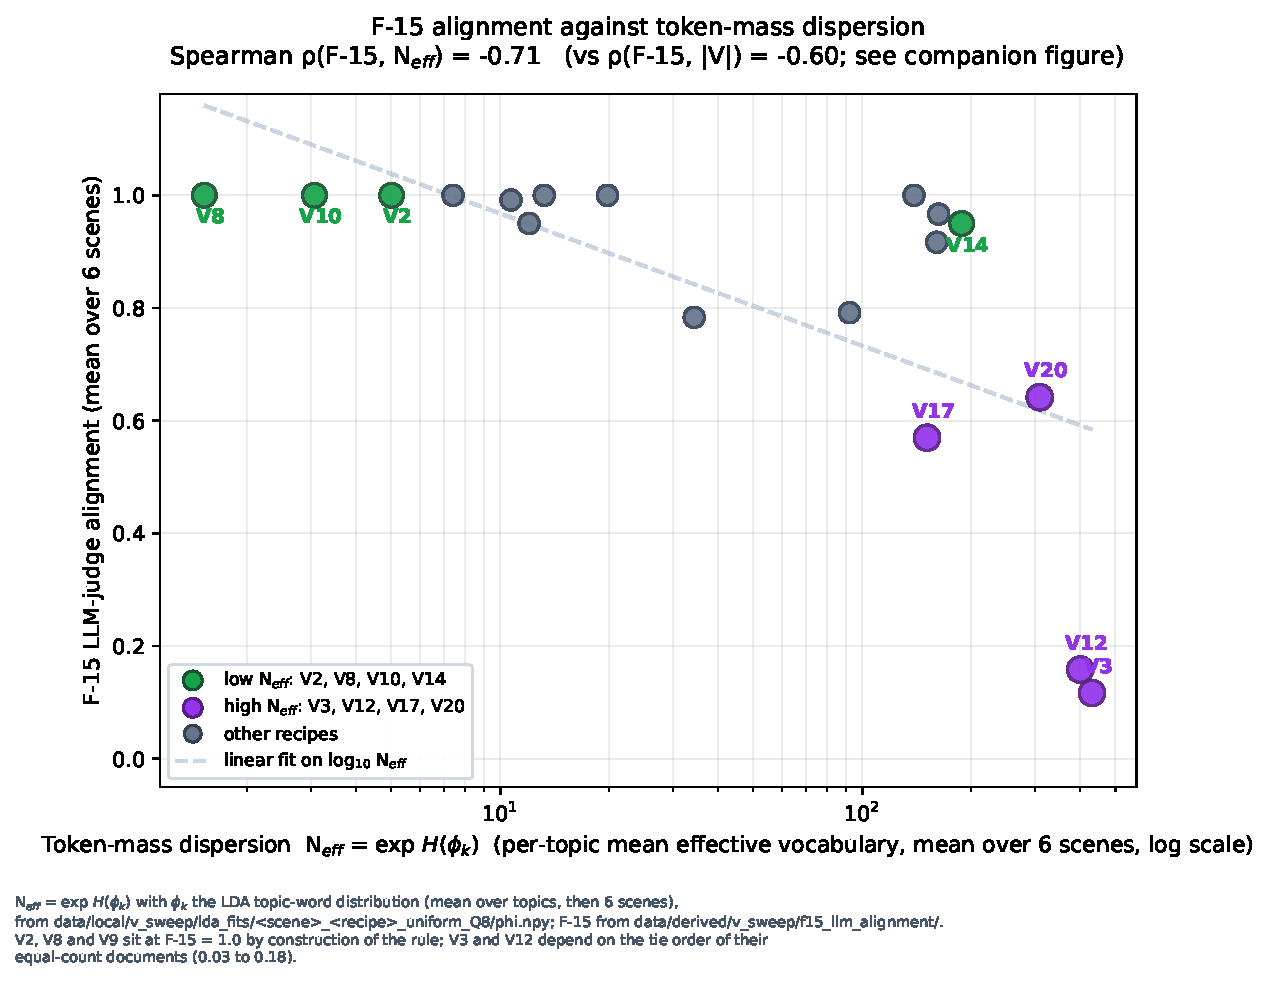
\includegraphics[width=\columnwidth]{p5-dispersion-scatter.pdf}
\caption{F-15 LLM-judge alignment versus per-topic mean
token-mass dispersion $N_{\mathrm{eff}}=\exp(H(\phi_k))$
\eqref{eq:dispersion}, LDA backbone, six labelled scenes, $Q=8$,
nineteen recipes (Table~\ref{tab:f15}); the Spearman coefficients in
the title are computed over the same nineteen, with average ranks for
tied values. Point colours are categorical: green for the low-$N_{\mathrm{eff}}$
recipes (V2, V8, V10, V14), purple for the high-$N_{\mathrm{eff}}$
recipes (V3, V12, V17, V20), grey for the others. At the same alphabet
size (mean nominal $|\mathcal{V}|\approx1376$), V3 / V12 / V20 (purple,
lower right) fall in dispersion ($431\!>\!400\!>\!309$) while F-15 is
$0.17$, $0.17$ and $0.65$; the V3 and V12 values are expectations over
tie orders, and V2, V8 and V9 sit at 1.0 by construction
(Table~\ref{tab:f15ties}), so the plotted association mixes dispersion
with the rule's construction effects.}
\label{fig:dispersion}
\end{figure}

\begin{figure}[t]
\centering
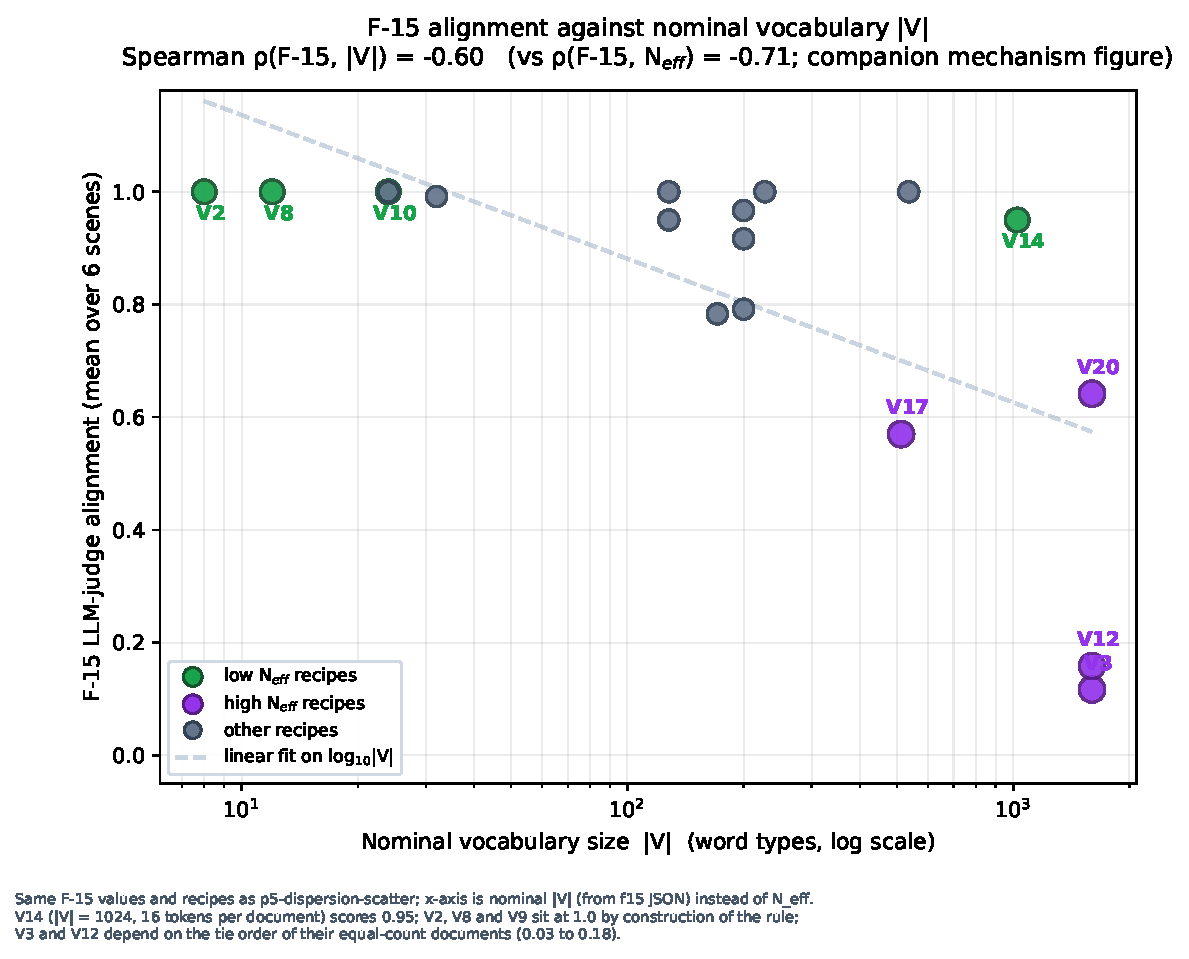
\includegraphics[width=\columnwidth]{p5-f15-vocab.pdf}
\caption{F-15 versus nominal vocabulary $|\mathcal{V}|$ (log scale),
nineteen recipes (Table~\ref{tab:f15}). A pure
vocabulary-size account would place all points on a monotone
decreasing curve. V14 ($|\mathcal{V}|=1024$, 16 tokens per document,
F-15 $=0.96$) and V20 ($|\mathcal{V}|\approx1376$, F-15 $=0.65$) sit far
above V3 / V12, so vocabulary size alone does not set F-15; V9
($|\mathcal{V}|=647$, F-15 $=1.0$) is fixed by the rule and is no
evidence either way.}
\label{fig:f15vocab}
\end{figure}

% =====================================================================
\section{Interpretability under the V13--V20 extension}
\label{sec:v13-v20-interp}
% =====================================================================

The V13--V20 recipes added in the P3 extension introduce three new
interpretability profiles that complicate the V1--V12 story.

\paragraph{V13 (VQ-VAE codebook) and V17 (sparse-coding dictionary)}
Both recipes produce \emph{opaque token alphabets}: the codeword
index does not map to a wavelength, an absorption feature, or a
band group. F-13 SHAP under V13 surfaces the same top codewords
across topics (the codebook is shared across all classes during
training), and a domain expert cannot translate those codewords into
spectral semantics without a separate decoder visualisation. We
classify V13 / V17 as the \emph{lowest-interpretability} branch of
the sweep: even when their F-13 SHAP is reportable, the explanation
is recursive: ``topic $k$ is dominated by codeword $c$, where
codeword $c$ is the centroid of pixels with [unrecoverable from
the recipe alone]''.

\paragraph{V14 (CWT-Morlet) and V18 (graph-Laplacian)}
The opposite case. V14 tokens are
\texttt{(log\_scale\_idx, position\_bucket, magnitude\_bin)};
each (scale, position) pair maps to a spectral region (one of eight
position buckets) at a bandwidth set by the scale (sixteen scales
from 1 to $B/2$ bands), and the bin quantises the wavelet magnitude.
On Indian Pines and Pavia~U the top SHAP tokens of every topic sit at
the three coarsest scales (\texttt{s13} to \texttt{s15}), so V14
explanations name broad spectral shape in a region rather than narrow
absorption features. V18 tokens are \texttt{(eigenvector\_id, bin)};
the eigenvector index names a mode of the kNN graph and the bin a
position along it. The top SHAP tokens of a V18 topic mix low- and
high-order modes (on Pavia~U, modes 0 to 14), so a V18 explanation
names positions on graph modes, which carry no spectral meaning
without a map of each mode back to pixels. V14 thus extends the
V1 + V7 physically-grounded profile to multi-scale spectral shape; V18
is grounded in the pixel graph rather than in the spectrum.

\paragraph{V19 (UMAP coords) and V15 (spectral indices)}
V15 is the easiest: top tokens of every topic map directly to
NDVI / MNDWI / NBR / NDSI / EVI / SAVI bins, with published
semantics. V19 has the inverse problem of V13: token names
\texttt{(axis\_0, q\_bin\_03)} are abstract coordinates with no
spectral anchor. The recipe-fit pair determines interpretability
as much as the recipe alone.

\paragraph{V20 (MI-weighted bands)}
V20 inherits V3's interpretability (its (band, q-bin) tokens are
spectrally grounded) and adds a label-aware twist \eqref{eq:v20}:
high-MI bands emit more copies than low-MI bands (on Indian Pines 169
of the 200 bands receive at least 5 of the 8 possible copies and one
band none), and its topics are less dispersed than V3's and V12's
($N_{\mathrm{eff}}$ 309 against 431 and 400, \S\ref{sec:f15}). Its SHAP
attributions are about as concentrated as V3's: the top token carries
0.28 of the top-8 mean $|$SHAP$|$ mass, against 0.26 for V3 and 0.27
for V12. V20 keeps V3's spectrally grounded vocabulary, adds label
information and needs no codebook, which makes it the most readable of
the extension recipes; its weights come from the labels of the same
pixels, so its explanations are label-informed by construction.

\paragraph{F-22 counterfactual under the extension}
Table~\ref{tab:f22-summary} already reports F-22 for all seven extension
recipes across the six labelled scenes at $Q=8$: V20, V12 and V3 form
the ultra-robust band (sentinel-patched means 26.3 / 24.5 / 23.5),
though, as noted in Section~\ref{sec:f22}, that ordering is dominated
by never-flipped scenes rather than a strict robustness gap. A full
F-22 across the $Q=16/32$ cross-product is left to a follow-up.

% =====================================================================
\section{Recommendation}\label{sec:rec}
% =====================================================================

For interpretability reporting, we recommend the following ordering:
\begin{enumerate}
  \item \textbf{F-13 SHAP attribution.} Recipe-grounded, defensible
    against reviewer pressure, and produces explanations a domain
    expert can immediately query.
  \item \textbf{F-22 counterfactual robustness.} Complements F-2/F-7
    by ruling out trivial-overfit explanations.
  \item \textbf{F-15 LLM-judge.} Only with its construction effects
    reported beside it (\S\ref{sec:f15}). The rule rewards small
    vocabularies and short documents and cannot judge one-token
    documents misaligned; its tie dependence is removed by taking the
    expectation over tie orders.
\end{enumerate}

The V13--V20 extension (\S\ref{sec:v13-v20-interp}) further suggests
a recipe-as-interpretability-tier classification:
\begin{itemize}
  \item \textbf{Tier I (physically-grounded)}: V1, V7, V14, V20.
    Top SHAP tokens map to a wavelength, absorption feature, scale
    band, or label-weighted band. Use for any publishable
    interpretability claim.
  \item \textbf{Tier II (semantically-grounded)}: V8, V10, V15.
    Top tokens map to endmember labels, group labels, or vegetation
    indices.
  \item \textbf{Tier III (learnt-codebook-grounded)}: V11, V12, V13,
    V17. Top tokens are codewords / GMM components / dictionary atoms.
    Interpretable only via a separate codebook-decoder visualisation.
  \item \textbf{Tier IV (manifold-coordinate)}: V18, V19. Topics point
    to kNN-graph modes or UMAP coordinates with no spectral anchor. Use
    only as a sanity baseline.
\end{itemize}

% =====================================================================
\section{Discussion}\label{sec:discussion}
% =====================================================================

\textbf{The three axes are complementary, not redundant.} F-13, F-22
and F-15 probe different facets of the same LDA fit. F-13 answers
\emph{which tokens explain a topic assignment}; F-22 answers
\emph{how robust that assignment is}; F-15 answers \emph{whether a
human-like judge would agree the document belongs to its topic}, a
question the current rule answers only through its construction
effects (\S\ref{sec:f15}). V20 shows how the axes can diverge: its
topics are less dispersed ($N_{\mathrm{eff}}$ 309 against 431 for V3),
its topics sit in the ultra-robust F-22 band (sentinel-patched mean
$=26.3$, with documents about six times longer than V3's), and P3 finds
it leads F-7 at $Q=32$, while its SHAP attributions are no more
concentrated than V3's. Whether these reflect one property of the MI
weighting is not tested here.

\textbf{F-15 measures the metric, not the model.} The central
methodological lesson is that an automated alignment proxy can fail
for reasons that have nothing to do with topic quality. The
anti-correlation between F-15 and F-2 on V3 / V12 is not evidence that
those recipes produce incoherent topics (P3 ranks V12 \emph{first}
on F-2 and F-7) but evidence that a top-$N$ identity-overlap rule is
governed by its construction: vocabulary size and tokens per document
(\S\ref{sec:f15}), and, unless ties are averaged out as they are here,
the order of tied counts. An actual LLM oracle, given
the same token lists and asked for identity overlap, would inherit the
same effects; only a judge equipped with
\emph{semantic} comparison of token meanings (e.g.\ the spectral
region a token names) would escape it. This is a cautionary result for
the growing practice of using LLMs to score topic models
\cite{stammbach2023revisiting}: the prompt must
expose token \emph{semantics}, not token \emph{strings}, or the score
will track vocabulary engineering rather than topic content.

\textbf{Interpretability is a recipe property, not an LDA property.}
The tier classification of \S\ref{sec:rec} shows that the same LDA
backbone yields explanations ranging from directly physical (V1, V7,
V14, V20) to recursively opaque or abstract (V13, V17, V18, V19). ``LDA is
interpretable'' is therefore an incomplete claim; the defensible claim
is ``LDA on a physically-grounded wordification is interpretable.''

% =====================================================================
\section{Limitations}\label{sec:limitations}
% =====================================================================

\textbf{LDA only.} Every result here is for the LDA backbone
\eqref{eq:lda-gen}. The closed-form posterior that makes F-13
tractable does not transfer unchanged to the two amortised neural
backbones of P4: the model labelled ProdLDA, which is the
mixture-decoder form (NVLDA) of Srivastava and Sutton's amortised topic
model~\cite{srivastava2017autoencoding} with a standard normal prior
\eqref{eq:prodlda-gen} (the product-of-experts decoder that defines
ProdLDA was not run), and ETM~\cite{dieng2020topic} \eqref{eq:etm-beta},
which shares that prior and encoder and differs only in its embedding
decoder; replicating these axes under P4's backbones is open work.

\textbf{Deterministic stand-in for the LLM oracle.} F-15 was produced by a
deterministic encoding of the alignment rule rather than by live
per-call LLM judging. This makes the run
reproducible and free, but it cannot exhibit the semantic-comparison
behaviour that a true oracle might; the API builder
(\path{build_v_sweep_f15_llm_alignment.py}) is provided for users
who wish to substitute live judging. Our claims about F-15 concern the
\emph{metric definition} \eqref{eq:f15} and its inputs (the top-$N$
token lists) and hold for any judge that receives those lists.

\textbf{$N_{\mathrm{eff}}$ is computed on $\phi_k$.} We measure
dispersion on the topic--word distributions, the quantity the
topic side of the F-15 rule reads; the canonical metric
\eqref{eq:dispersion} is stated on a generic mass vector $p_d$ and
applies equally to per-document counts, which the document side of the
rule reads and which this study does not summarise.

\textbf{Partial F-22 under the extension.} The full F-22 table
(Table~\ref{tab:f22-summary}) is complete for the $Q=8$ sweep, but the
$\times Q \times$ extension-recipe cross-product (\S\ref{sec:v13-v20-interp})
is profiled only spot-wise; a full re-run is left to a follow-up.

\textbf{Six labelled scenes.} The HIDSAG mineralogical subsets used in
P1~\cite{santibanezleal2026framework} are not included here because
their per-pixel label structure differs; the F-15 results should be
re-checked on them before being claimed as scene-independent.

% =====================================================================
\section{Conclusion}\label{sec:conclusion}
% =====================================================================

We instantiated three post-hoc interpretability axes (F-13 SHAP
attribution, F-22 counterfactual $L_1$, and F-15 LLM-judge alignment)
on the LDA wordification sweep of P3, and reported three results.
First, F-13 SHAP gives recipe-grounded explanations whose physical
meaning is fixed by the recipe and cannot silently shift across scenes;
this is the axis we recommend as the primary interpretability artefact.
Second, F-22 separates the recipes into an ultra-robust band (V20 / V12 /
V3, sentinel-patched means 26.3 / 24.5 / 23.5, in which most documents
never flip within 50 steps) and a fragile regime (V9 $=1.0$); F-22
grows with the document length, which this ordering partly reflects.
Third, and most important methodologically, F-15 as defined is
governed by construction effects of its top-10 overlap rule rather
than by agreement between documents and topics: it is 1.0 by
construction for small vocabularies (V2, V8) and one-token documents
(V9), and near 1.0 for three- and four-token documents. For recipes
whose documents hold every token once (V3, V12) no sort order is
informative, so we report the expectation over tie orders (0.167 and
0.171) instead of one draw between 0.03 and 0.18. V20 stays far above
V3 and V12 under every tie order and has less dispersed topics
($N_{\mathrm{eff}}$ 309 against 431 and 400), but its copies also rank
the tokens of its documents, so the gap cannot be attributed to topic
dispersion. We therefore recommend reporting F-15 only with these
construction effects beside it, and we caution that LLM-as-judge topic
evaluation inherits them unless the judge is given token
\emph{semantics} rather than token strings. Extending these axes across
the P4 backbones, and re-checking the F-15 results on the HIDSAG
subsets, are the natural next steps.

\medskip
\noindent\textbf{Declaration of generative AI use.} Generative AI tools
were used for formulating the alignment rule that stands in for the LLM
oracle of the F-15 axis, applied as a deterministic function. The author
reviewed and verified all content and takes full responsibility for the
work.

% =====================================================================
\bibliographystyle{IEEEtran}
\bibliography{../../bibliography/refs,companion}

\end{document}
